\documentclass[10pt]{article}
\usepackage[margin=0.5in]{geometry}
\usepackage{epsfig}

\begin{document}

\section{How often do shelters need to be cleaned?}

\begin{figure}
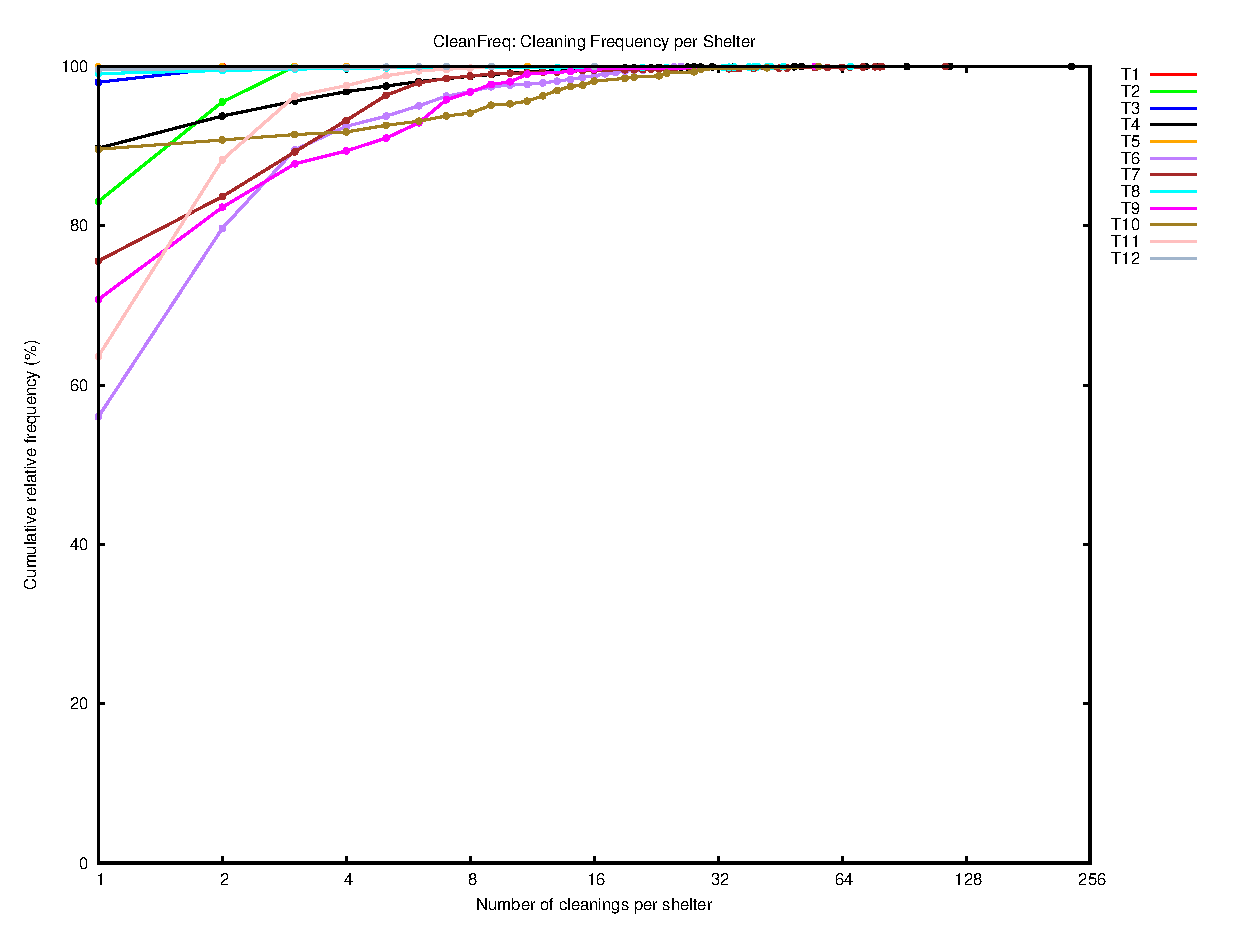
\includegraphics[scale=2, width=\textwidth]{freq.eps}
\end{figure}


\subsection{Comments on Cleaning Frequency}
In every trace, the vast majority of shelters must be cleaned only a few times. 
Except in the TPCE/TPCC traces, most shelters are never cleaned at all,
and in every case, over 80\% of the shelters are cleaned 3 times or fewer.
Although this graph doesn't show it,  a few especially busy shelters 
may be cleaned tens or even hundreds of times.
For example, one shelter in trace 4 is cleaned 231 times. 
However, this is uncommon.

\clearpage

\begin{figure}
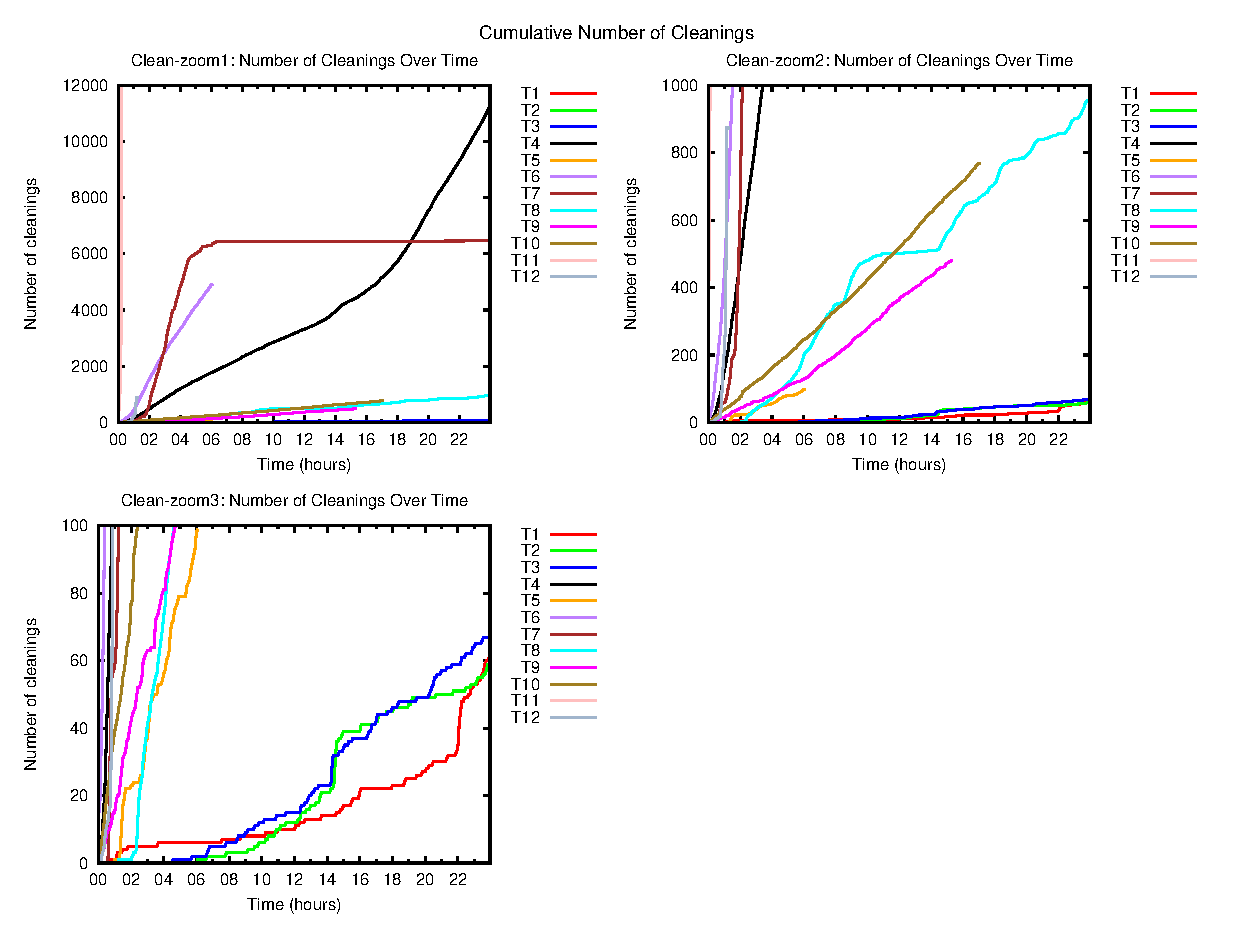
\includegraphics[scale=2, width=\textwidth]{cum_freq.eps}
\end{figure}

\subsection{Comments on Cumulative Number of Cleanings}
The graph of cumulative number of cleanings shows that very few cleanings are
required overall. The traces that require far more cleanings (T4, T6, T7
and T12) have far more requests overall; in general, number of cleanings 
roughly map sto total number of requests (or rather, total number of writes).
This means the overhead in disk activity from swapping shelters to other locations
will be quite low. The additional requests required to clean come out to a fraction
of a percent of total number requests for T4 and T7, and I suspect for other traces as
well. However, plotting total number of cleanings as a percentage of total number of 
requests might be helpful. 

\clearpage

\section{Will we run out of empty shelters?}

The graphs below illustrate that we run out of empty shelters quite infrequently; 
only four disks need to be reset at any point, and none need to be reset more than once.
These results are also based on the assumption that the disk is full; 
specifically, we assume that there is one additional shelter after the last block accessed in the trace.
This assumption is extremely conservative,
and is likely causing us to greatly underestimate the number of shelters available
on mostly-empty disks.

For instance, in T4, disk0 requires a reset around 22 hours,
when about 1000 shelters are full
Since we preallocate a shelter every 100 MB, 
this would mean the total disk size is around 100MB * 1000,
which comes out to under 100 GB.
In fact, each disk used in T4 is a RAID array of at least 292GB,
meaning roughly 2000 more shelters would be available to us,
and a reset would not actually be necessary.

Similarly, we can see that disk4 and disk5 in T6 both reset
around 1600 shelters, which would suggest that both disks
have about 160 GB total capacity.
While we do not have information about the actual disk sizes in T6,
it seems unlikely that they are this small. 
T6, disk0 and T10, disk0, the other two that need to be reset,
would have to be even smaller.

In short, it is likely that if we could take their actual size into account
instead of conservatively assuming they are full,
none of the disks here would come anywhere near running out of free shelter space.

\begin{figure}
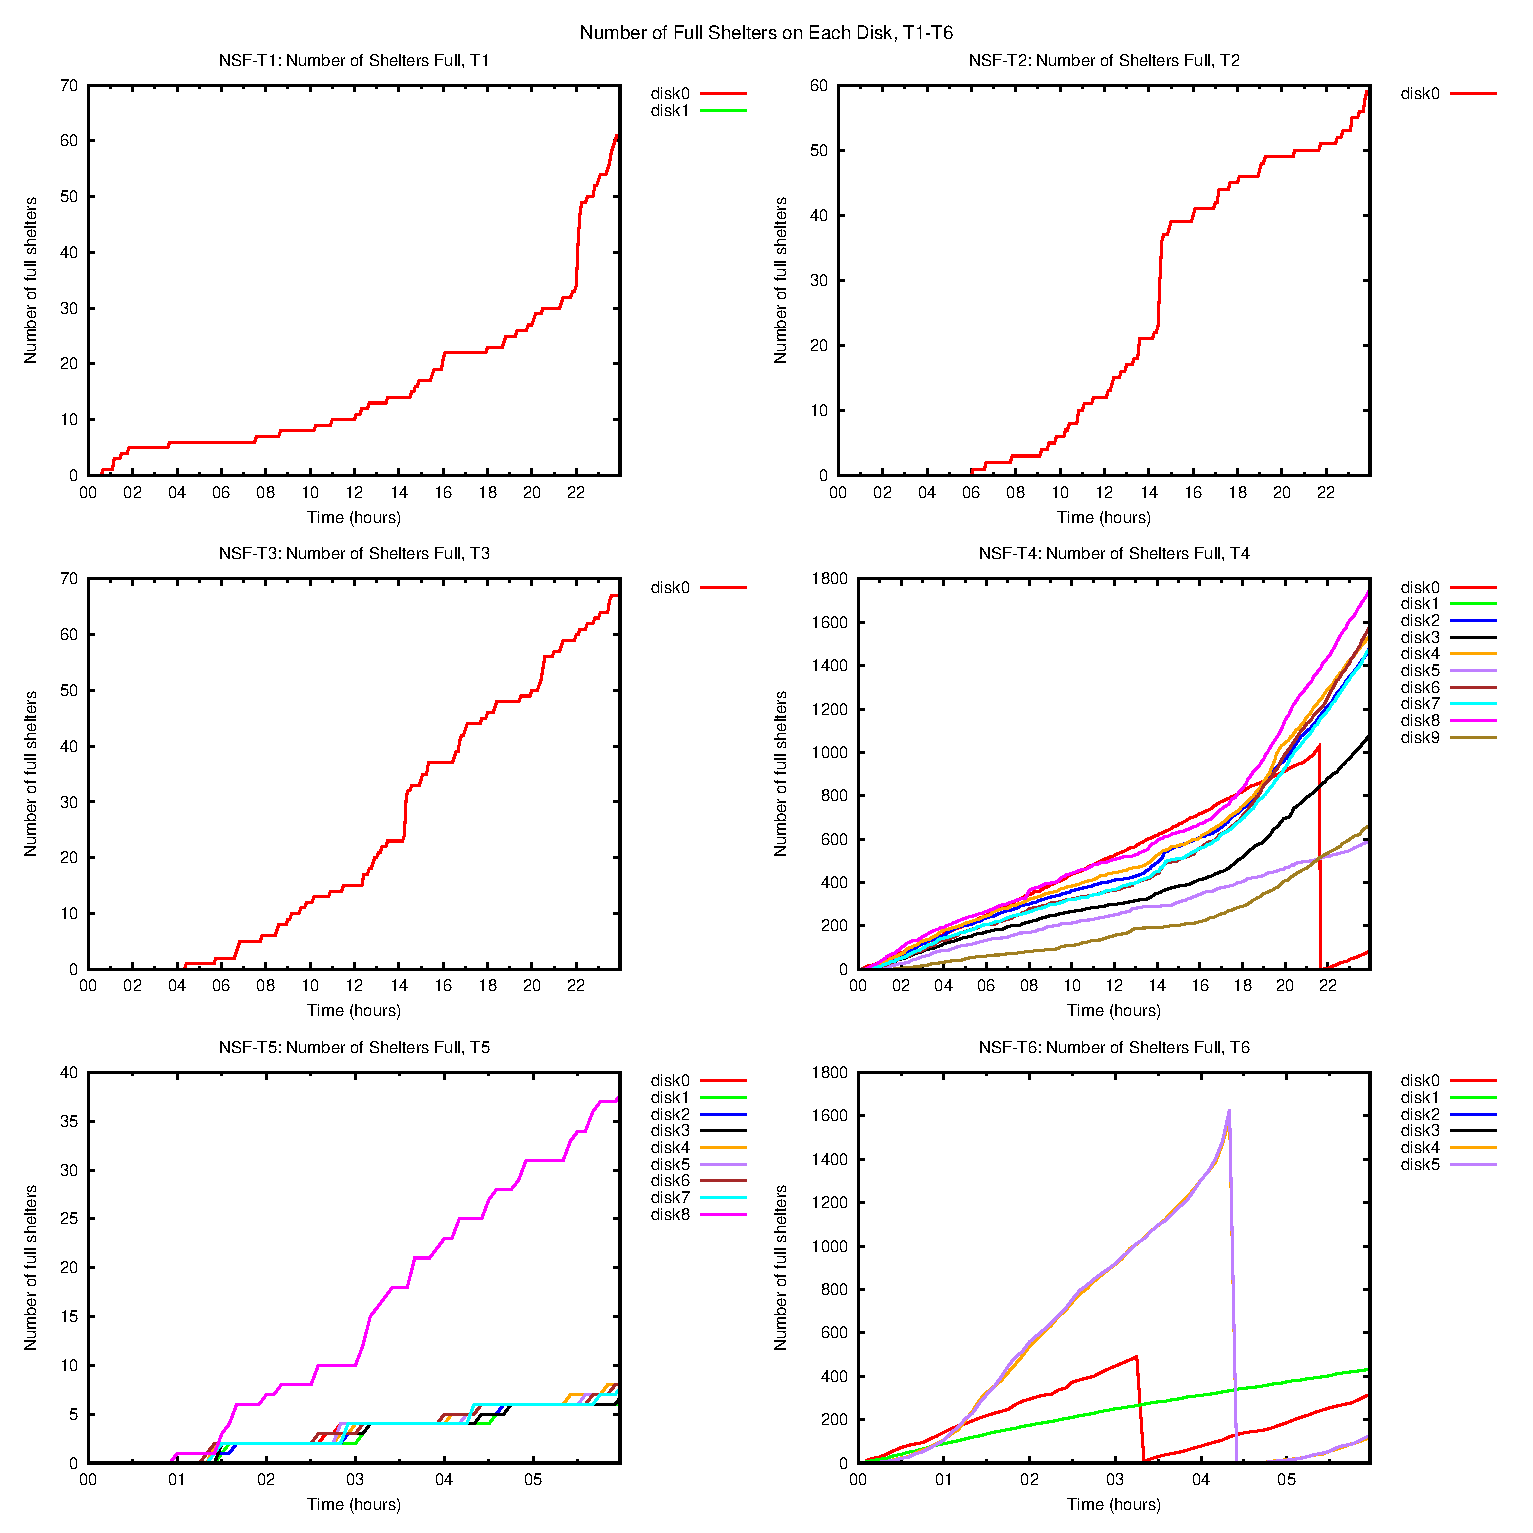
\includegraphics[scale=2, width=\textwidth]{full_shelt_cnt1.eps}
\end{figure}

\begin{figure}
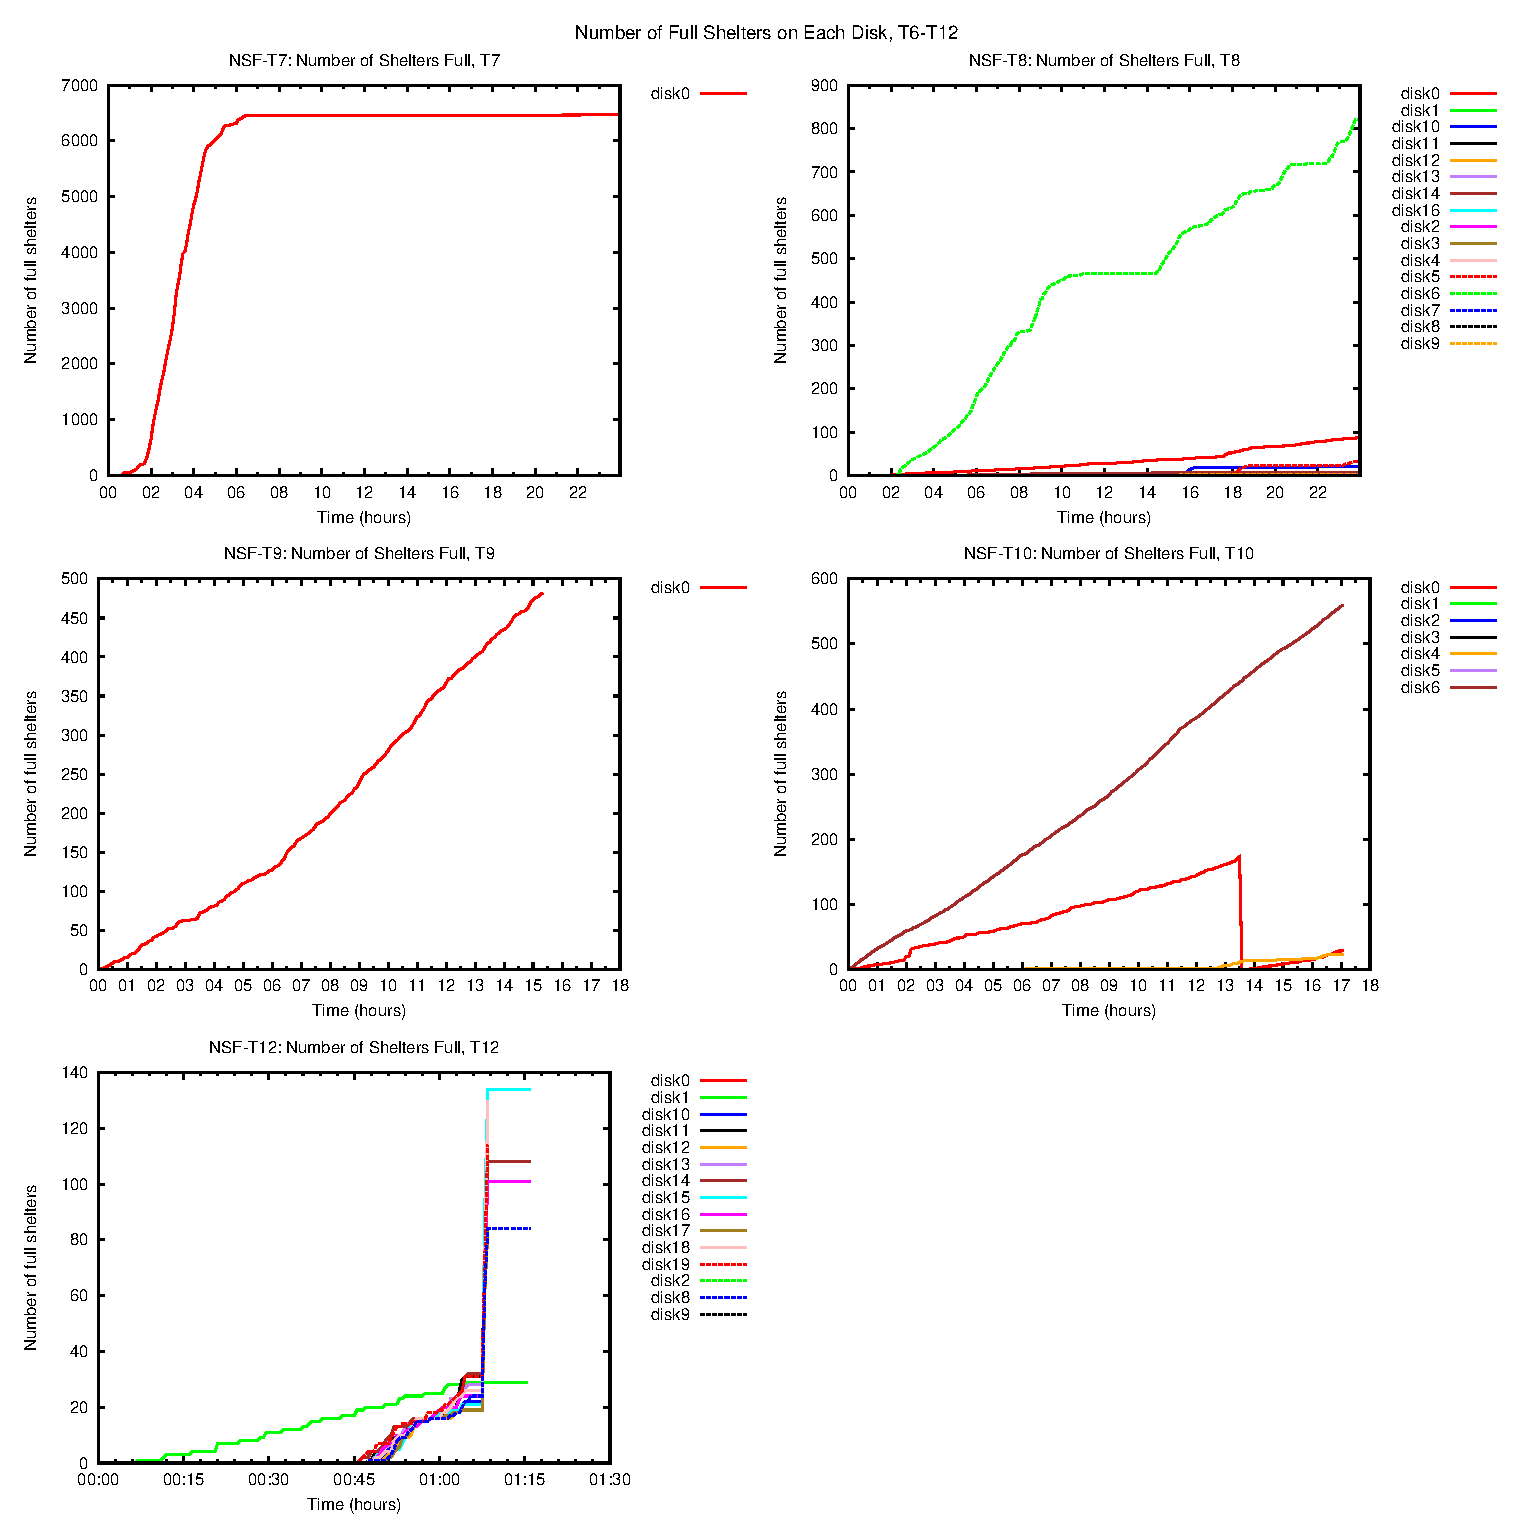
\includegraphics[scale=2, width=\textwidth]{full_shelt_cnt2.eps}
\end{figure}

\begin{figure}
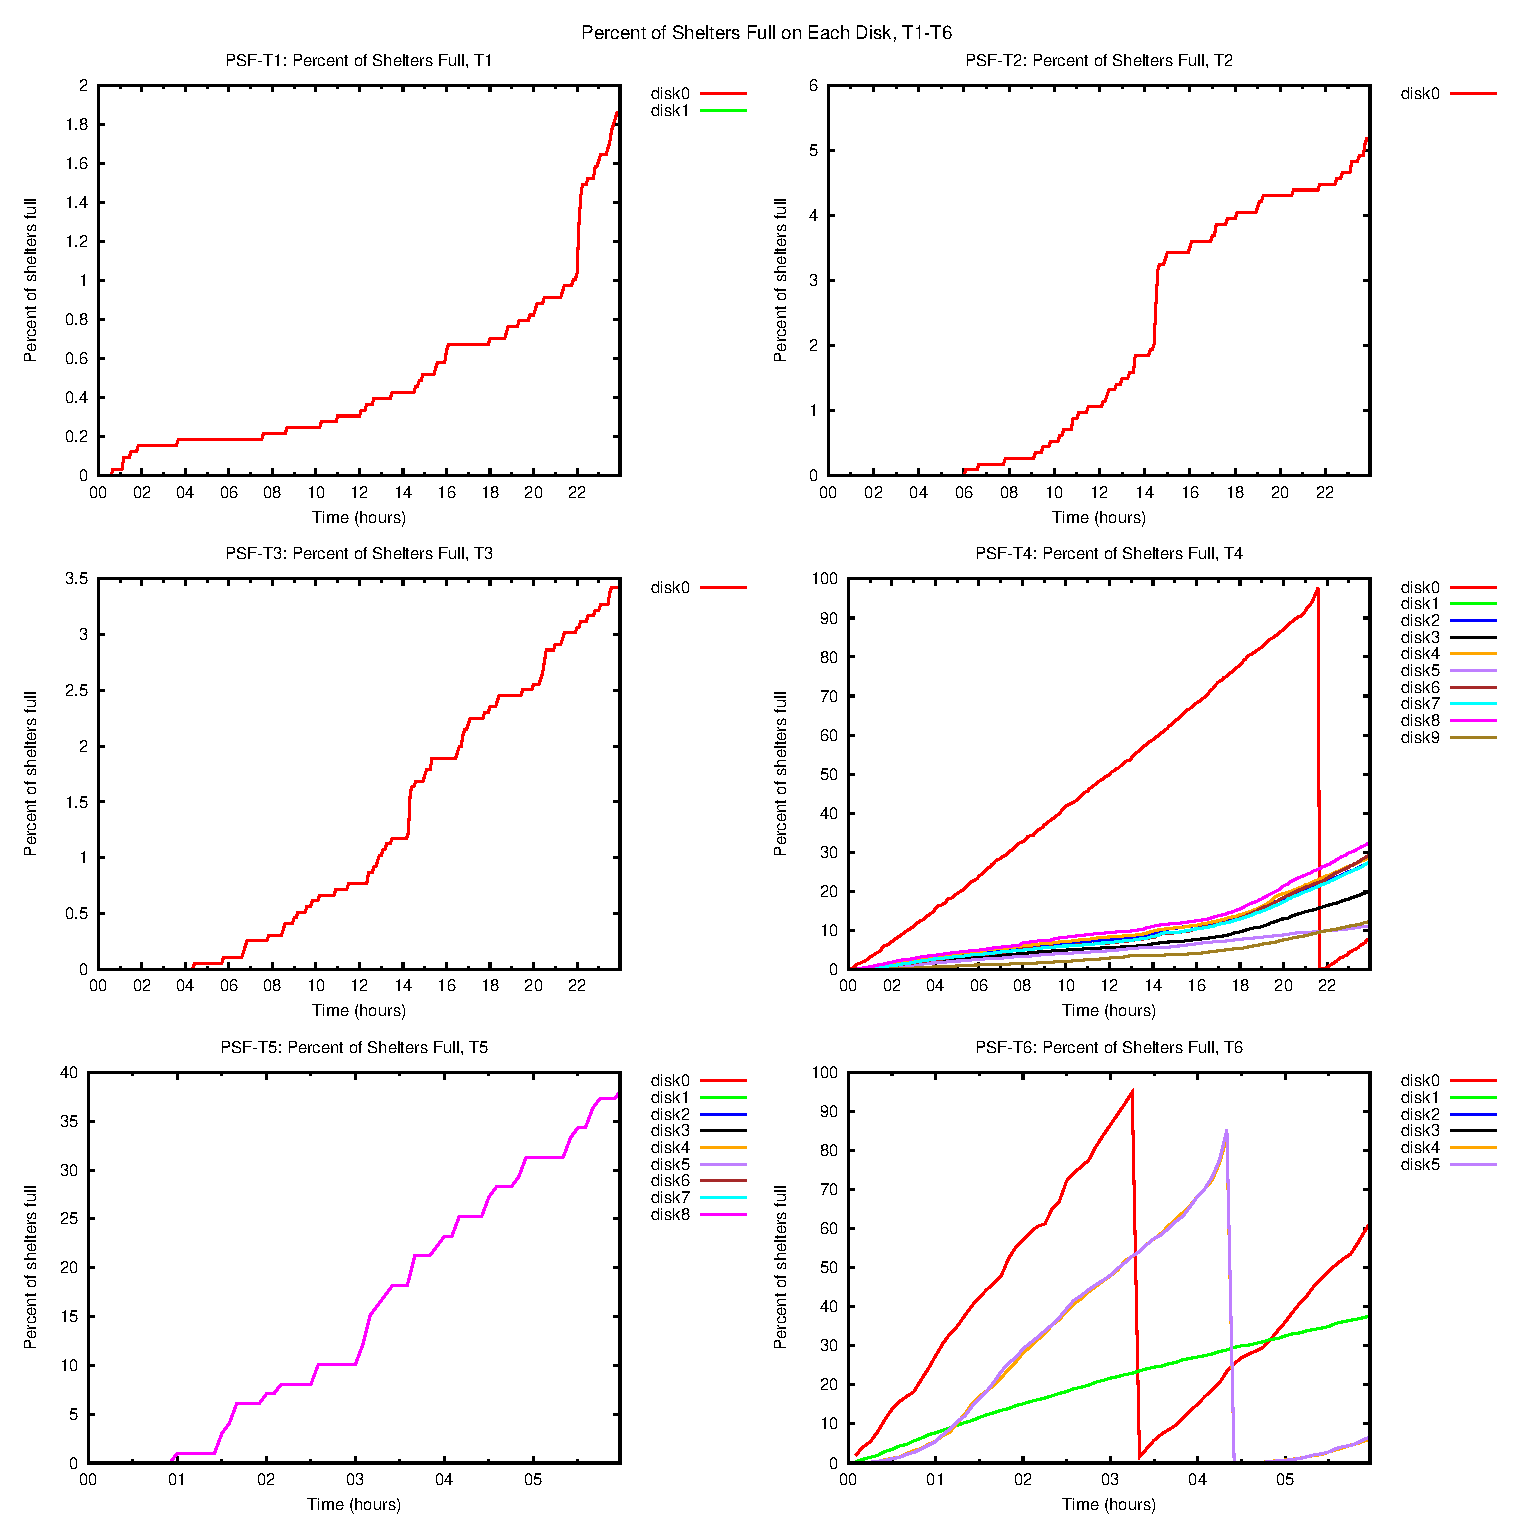
\includegraphics[scale=2, width=\textwidth]{full_shelt_percent1.eps}
\end{figure}

\begin{figure}
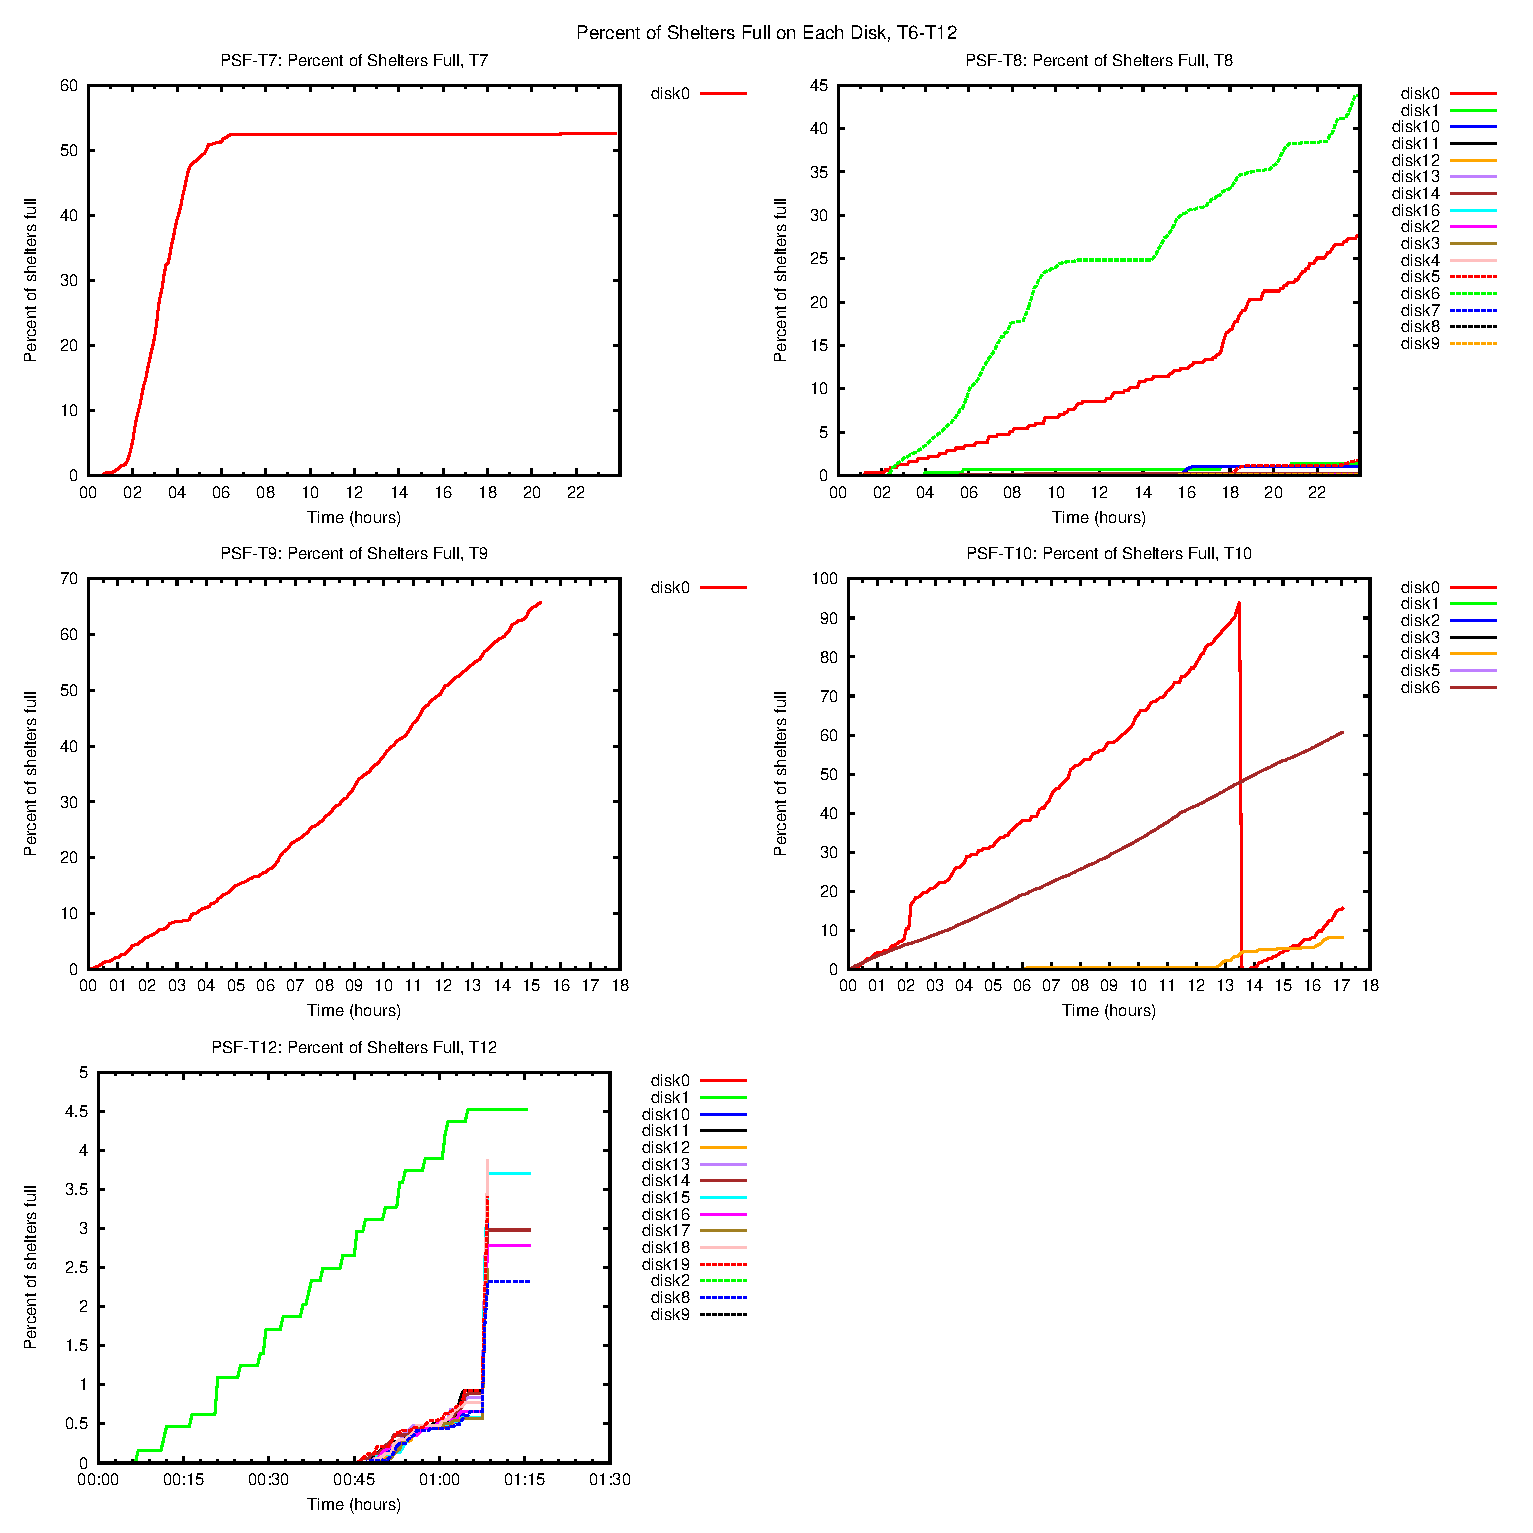
\includegraphics[scale=2, width=\textwidth]{full_shelt_percent2.eps}
\end{figure}

\clearpage

\section{Do we have enough memory to keep pointers to all sheltered blocks?}

When a block is sheltered, we need to track its actual location on disk.
That means we'll need a lookup table mapping final block locations to sheltered block locations.
To get a sense of how large this table would need to be, 
the graphs above track the number of unique sheltered blocks for each trace.
Unsurprisingly, this tracks pretty closely with C-32-W, the graph tracking the total size of all sheltered data.
They are measuring the same thing, but here we take into account that sheltered blocks can be overwritten,
in which case we don't need to track the old and new block.

The lookup table for block locations will require two words per entry (one for the final block location, one for the sheltered block location),
so each entry will be 16 bytes on a 32-bit architecture.
Of course, this is a lower bound--this particular table structure wouldn't actually work because it doesn't allow fast lookups.
At most, we would need about 16 million entries, for T7, the Windows build server. This would require about 250 MB.
T4, the Exchange server; T12, the TPCE benchmark; and T6, the MSN file server, would also require relatively large lookup tables,
of roughly 150MB, 135MB, and 90 MB, respectively. 
The remaining entries would require lookup tables of less than about 30 MB, and most far less than that.

\begin{figure}
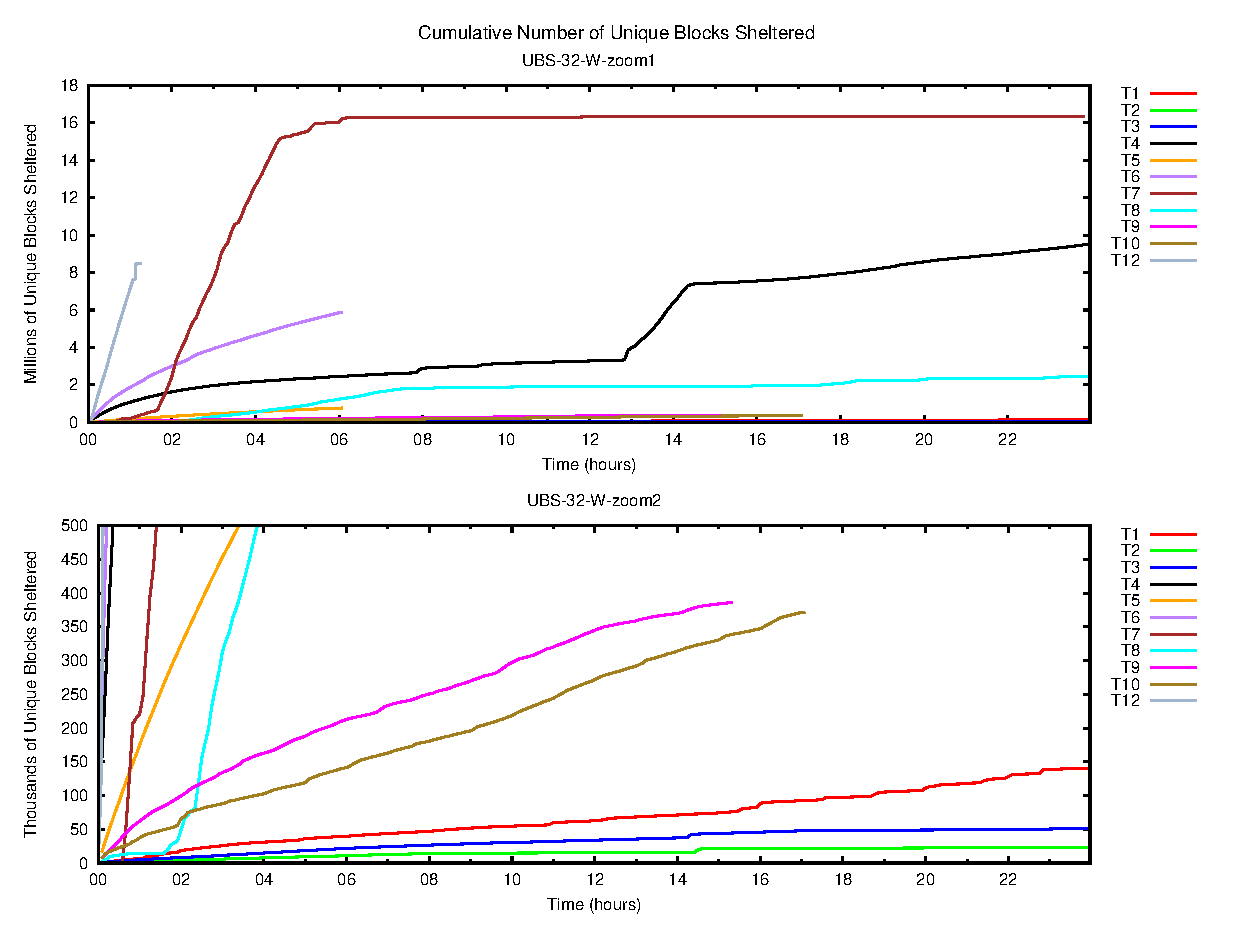
\includegraphics[scale=2, width=\textwidth]{ptr_cnt.eps}
\end{figure}

\section{Which writes should be sheltered?}

The graphs below give a general overview of the size distribution of read and write requests, 
and suggest that, for most traces, the bulk of small requests are smaller than 8KB,
so an 8KB cutoff might make sense.

The DSPH graphs suggest that most traces are not very bursty;
except for T7, the average and maximum amount of data sheltered per hour are pretty similar.
(In many cases, no hour was clearly the busiest, so the hour sampled was more or less arbitrary.)

\begin{figure}
  \centering
  \begin{minipage}{.5\textwidth}
    \centering
    \includegraphics[width=.95\linewidth]{../c_results/PIO-All-W.eps}
  \end{minipage}%
  \begin{minipage}{.5\textwidth}
    \centering
    \includegraphics[width=.95\linewidth]{../c_results/PIO-All-R.eps}
  \end{minipage}

  \begin{minipage}{.5\textwidth}
    \centering
    \includegraphics[width=.95\linewidth]{../c_results/PS-All-W.eps}
  \end{minipage}%
  \begin{minipage}{.5\textwidth}
    \centering
    \includegraphics[width=.95\linewidth]{../c_results/PS-All-R.eps}
  \end{minipage}
\end{figure}

\begin{figure}
  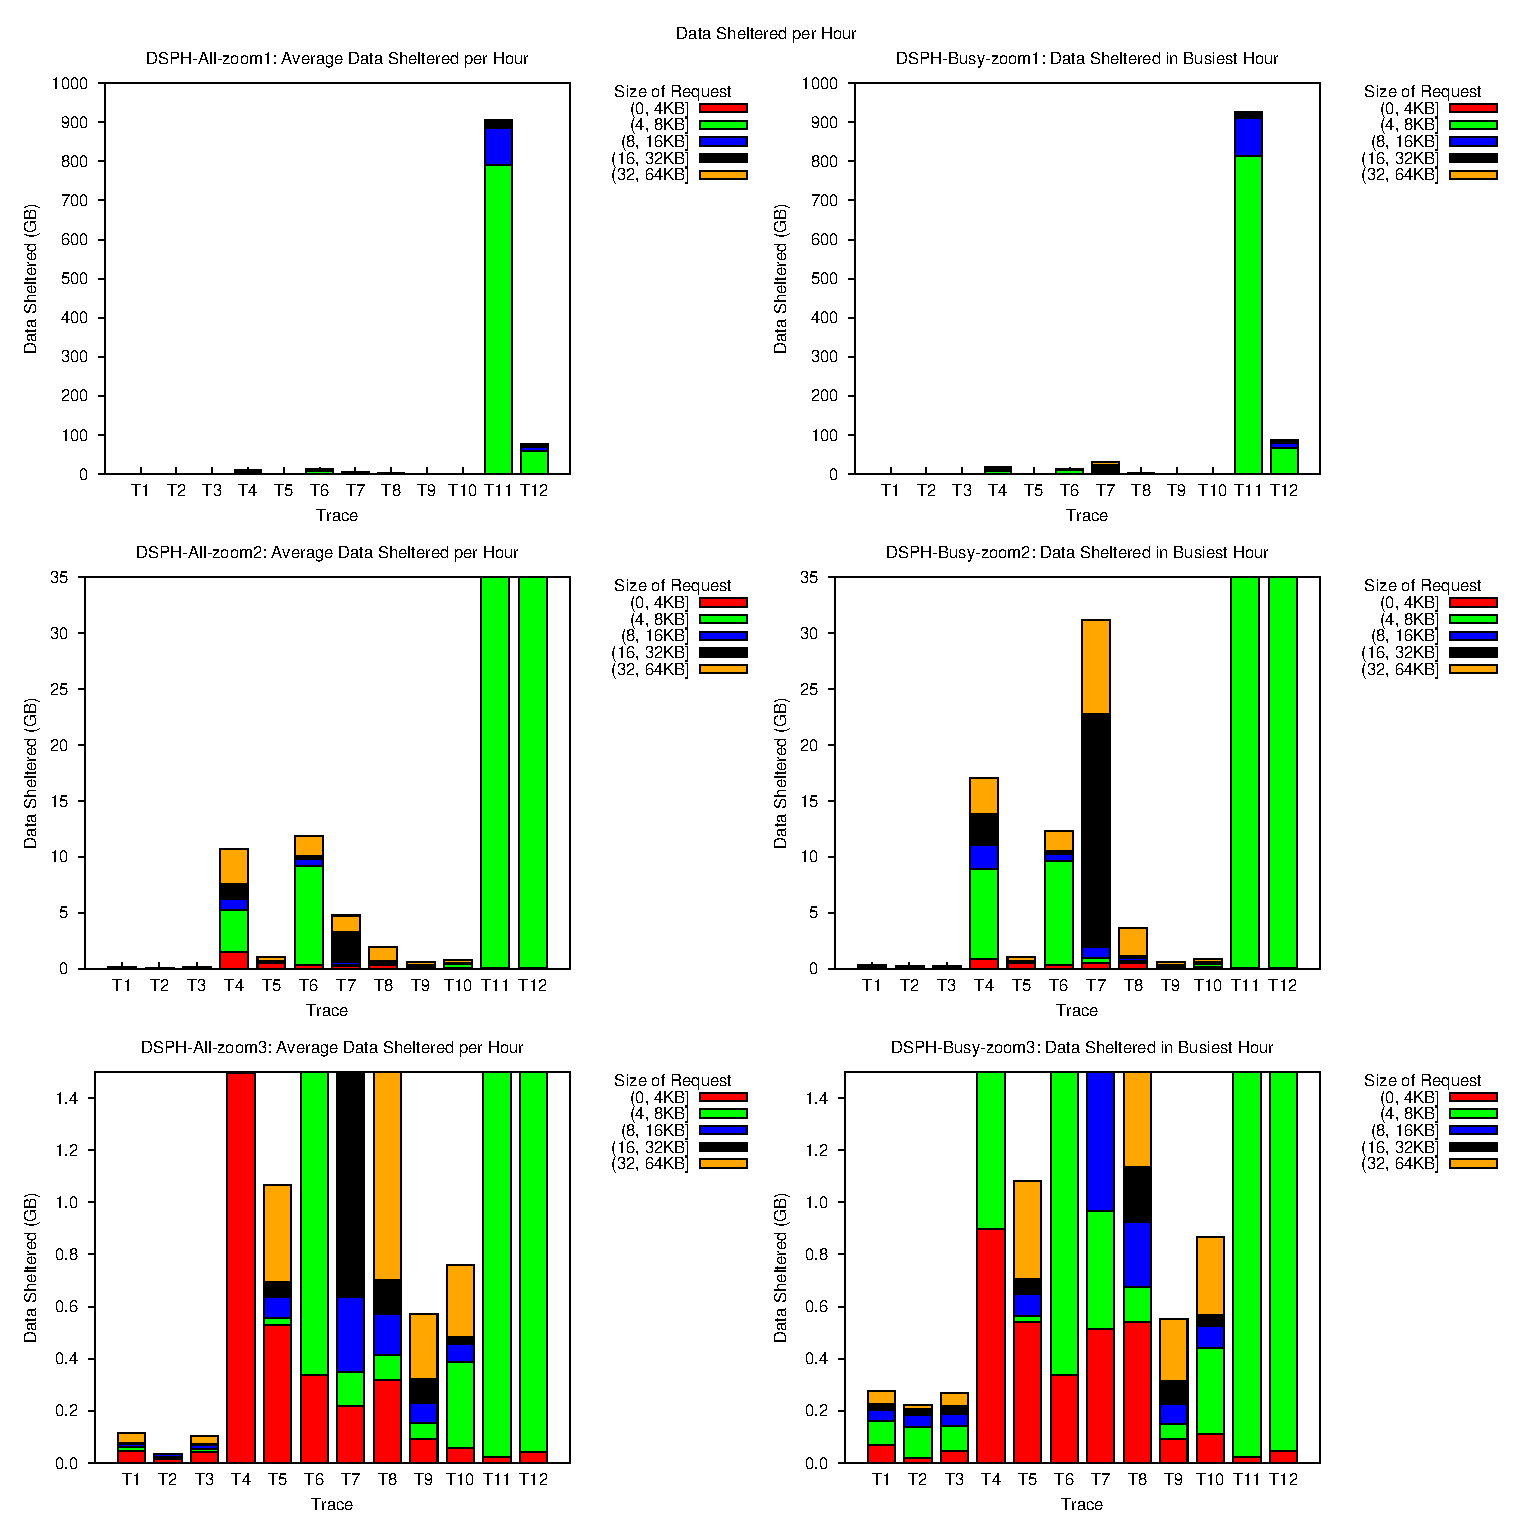
\includegraphics[width=\textwidth]{../c_results/DSPH.eps}
\end{figure}

\end{document}
